%!TEX program = xelatex
\documentclass[dvipsnames, svgnames,a4paper,11pt]{article}
% ----------------------------------------------------
%   中山大学物理与天文学院本科实验报告模板
%   作者:Huanyu Shi,2019级
%   知乎:https://www.zhihu.com/people/za-ran-zhu-fu-liu-xing
%   Github:https://github.com/Huanyu-Shi/SYSU-SPA-Labreport-Template
%   Last update : 2023.4.10
% ----------------------------------------------------

% ----------------------------------------------------- 
%	加边框的命令
%	参考:https://tex.stackexchange.com/questions/531559/how-to-add-the-page-border-for-first-two-pages-in-latex
\usepackage{tikz}
\usetikzlibrary{calc}
\usepackage{eso-pic}
\AddToShipoutPictureBG{%
\begin{tikzpicture}[overlay,remember picture]
\draw[line width=0.6pt] % 边框粗细
    ($ (current page.north west) + (0.6cm,-0.6cm) $)
    rectangle
    ($ (current page.south east) + (-0.6cm,0.6cm) $); % 边框位置
\end{tikzpicture}}


\usepackage{xcolor}
\definecolor{c1}{HTML}{2752C9} % 目录颜色
\definecolor{c2}{RGB}{190,20,83} % 引用颜色

\usepackage{ctex}
\usepackage[top=28mm,bottom=28mm,left=15mm,right=15mm]{geometry}
\usepackage{hyperref} 
\hypersetup{
	colorlinks,
	linktoc = section, % 超链接位置,选项有section, page, all
	linkcolor = c1, % linkcolor 目录颜色
	citecolor = c1  % citecolor 引用颜色
}
\usepackage{amsmath,enumerate,multirow,float}
\usepackage{tabularx}
\usepackage{tabu}
\usepackage{subfig}
\usepackage{fancyhdr}
\usepackage{graphicx}
\usepackage{wrapfig}  
\usepackage{physics}
\usepackage{appendix}
\usepackage{amsfonts}

%
\usepackage{tcolorbox}
\tcbuselibrary{skins,breakable}
\newtcolorbox{tbox}[2][]{
    colframe=black!70!,
    breakable,
    enhanced,
	boxrule =0.5pt,
    title = {#2},
    fonttitle = \large\kaishu\bfseries,
	drop fuzzy shadow,
    #1
}
\newtcolorbox[auto counter,number within=section]{question}[1][]{
  top=2pt,bottom=2pt,arc=1mm,
  boxrule=0.5pt,
%   frame hidden,
  breakable,
  enhanced, %跨页后不会显示下边框
  coltitle=c1!80!gray,
  colframe=c1,
  colback=c1!3!white,
  drop fuzzy shadow,
  title={思考题~\thetcbcounter:\quad},
  fonttitle=\bfseries,
  attach title to upper,
  #1
}
\newcommand{\setLhead}[1]{%
  \lhead{{\color{gray}\kaishu #1}} % 定义新的命令,设置右边页眉的内容
}
\newcommand{\setRhead}[1]{%
  \rhead{{\color{gray}\kaishu #1}} % 定义新的命令,设置右边页眉的内容
}
% ---------------------------------------------------------------------
%	利用cleveref改变引用格式,\cref是引用命令
\usepackage{cleveref}
\crefformat{figure}{#2{\textcolor{c2}{图 #1}}#3} % 图片的引用格式
\crefformat{equation}{#2{(\textcolor{c2}{#1})}#3} % 公式的引用格式
\crefformat{table}{#2{\textcolor{c2}{表 #1}}#3} % 表格的引用格式


% ---------------------------------------------------------------------
%	页眉页脚设置
\fancypagestyle{plain}{\pagestyle{fancy}}
\pagestyle{fancy}
\setLhead{中山大学物理与天文学院基础物理实验预习报告}
%\lhead{\kaishu 中山大学物理与天文学院物理实验\uppercase\expandafter{\romannumeral3}} % 左边页眉,学院 + 课程
%\rhead{{\color{gray}\kaishu Template 实验报告模板}} % 右边页眉,实验报告标题
\setRhead{实验1\hspace{1pt}冰的熔化热测量}
\cfoot{\thepage} % 页脚,中间添加页码


% ---------------------------------------------------------------------
%	对目录、章节标题的设置
\renewcommand{\contentsname}{\centerline{\huge 目录}}
\usepackage{titlesec}
\usepackage{titletoc}
% \titleformat{章节}[形状]{格式}{标题序号}{序号与标题间距}{标题前命令}[标题后命令]
\titleformat{\section}{\centering\LARGE\songti}{}{1em}{}

% ---------------------------------------------------------------------
%   listing代码环境设置
\usepackage{listings}
\lstloadlanguages{python}
\lstdefinestyle{pythonstyle}{
backgroundcolor=\color{gray!5},
language=python,
frameround=tftt,
frame=shadowbox, 
keepspaces=true,
breaklines,
columns=spaceflexible,                   
basicstyle=\ttfamily\small, % 基本文本设置,字体为teletype,大小为scriptsize
keywordstyle=[1]\color{c1}\bfseries, 
keywordstyle=[2]\color{Red!70!black},   
stringstyle=\color{Purple},       
showstringspaces=false,
commentstyle=\ttfamily\scriptsize\color{green!40!black},%注释文本设置,字体为sf,大小为smaller
tabsize=2,
morekeywords={as},
morekeywords=[2]{np, plt, sp},
numbers=left, % 代码行数
numberstyle=\it\tiny\color{gray}, % 代码行数的数字字体设置
stepnumber=1,
rulesepcolor=\color{gray!30!white}
}




% ---------------------------------------------------------------------
%	其他设置
\def\degree{${}^{\circ}$} % 角度
\graphicspath{{./images/}} % 插入图片的相对路径
\allowdisplaybreaks[4]  %允许公式跨页 % 导入模板的相关设置
\usepackage{lipsum}
\usepackage{indentfirst}
\usepackage{pdfpages}
\usepackage{multirow}
\usepackage{subfig}
\usepackage{graphicx}
\usepackage{float} 
\usepackage{booktabs}
\usepackage{enumerate}
\usepackage{makecell} 
\renewcommand{\d}{\mathrm{d}}
\newcommand{\upcite}[1]{\textsuperscript{\textsuperscript{\cite{#1}}}}


%---------------------------------------------------------------------
%	正文
%---------------------------------------------------------------------
\newcommand{\exname}{基本电路元件伏安特性的测量}%实验名称
\setRhead{\exname}
\begin{document}


\begin{table}
	\renewcommand\arraystretch{1.7}
	\begin{tabularx}{\textwidth}{
		|X|X|X|X
		|X|X|X|X|}
	\hline
	\multicolumn{2}{|c|}{预习报告}&\multicolumn{2}{|c|}{实验记录}&\multicolumn{2}{|c|}{分析讨论}&\multicolumn{2}{|c|}{总成绩}\\
	\hline
	 \hspace{0.625cm}25& & \hspace{0.625cm}35  & & \hspace{0.625cm}30  & &  \hspace{0.625cm}90 & \\
	\hline
	\end{tabularx}
\end{table}


\begin{table}
	\renewcommand\arraystretch{1.7}
	\begin{tabularx}{\textwidth}{|X|X|X|X|}
	\hline
	年级、专业:& 2023级物理学类 &组号:& \\
	\hline
	姓名:& 姚昊廷  & 学号:&22322091\\
	\hline
	日期:& & 教师签名:& \\
	\hline
	\end{tabularx}
\end{table}

\begin{center}
	\LARGE \exname
\end{center}

\textbf{【实验报告注意事项】}
\begin{enumerate}
	\item 实验报告由三部分组成:
	\begin{enumerate}
		\item 预习报告:课前认真研读\underline{\textbf{实验讲义}},弄清实验原理;实验所需的仪器设备、用具及其使用、完成课前预习思考题;了解实验需要测量的物理量,并根据要求提前准备实验记录表格。
	    \item 实验记录:认真、客观记录实验条件、实验过程中的现象以及数据。实验记录请用珠笔或者钢笔书写并签名(\textcolor{red}{\textbf{用铅笔记录的被认为无效}})。\textcolor{red}{\textbf{保持原始记录,包括写错删除部分,如因误记需要修改记录,必须按规范修改。}}(不得手记的值输入到电脑打印);离开前请实验教师检查记录并签名。
	    \item 数据处理及分析讨论:处理实验原始数据(学习仪器使用类型的实验除外),对数据的可靠性和合理性进行分析;按规范呈现数据和结果(图、表),包括数据、图表按顺序编号及其引用;分析物理现象(含回答实验思考题,写出问题思考过程,必要时按规范引用数据);最后得出结论。
	\end{enumerate}
	\textbf{实验报告就是将预习报告、实验记录、和数据处理与分析合起来,加上本页封面。}
	\item 实验报告在\textcolor{red}{\textbf{每个小结(补做)的之后一周内}}提交,最后一次实验,在\textcolor{red}{\textbf{结束一周内}}提交。
	\item 注意事项:\begin{enumerate}
		\item 请认真查看并理解\textcolor{red}{\textbf{实验讲义第一章}}内容
		\item 注意实验器材的合理使用。
		\item 使用结束使用各种仪器之后需要将其放回原位
	\end{enumerate}
\end{enumerate}



\clearpage
\tableofcontents
\clearpage

\setcounter{section}{0}
\section{\exname\ \textbf{预习报告}}
	
\subsection{实验目的}

\subsection{仪器用具}
\begin{table}[htbp]
	\centering
	\renewcommand\arraystretch{1.6}
	% \setlength{\tabcolsep}{10mm}
	\begin{tabular}{p{0.05\textwidth}|p{0.20\textwidth}|p{0.05\textwidth}|p{0.5\textwidth}}
	\hline
	编号& 仪器用具名称 & 数量 &  主要参数(型号,测量范围,测量精度等) \\
	\hline
	1&透镜LC&1 &\\
	\hline
\end{tabular}
\end{table}


\subsection{原理概述}
\subsection{实验预习题}
\begin{question}
    
\end{question}

\clearpage
\setLhead{中山大学物理与天文学院基础物理实验记录}
\begin{table}
	\renewcommand\arraystretch{1.7}
	\centering
	\begin{tabularx}{\textwidth}{|X|X|X|X|}
	\hline
	专业:& 物理学类 &年级:& 2023级 \\
	\hline
	姓名: &姚昊廷& 学号:&22322091  \\
	\hline
	室温:&$22^\circ$C&实验地点:&A508  14\\
	\hline
	学生签名:& & 评分: &\\
	\hline
	实验时间:& & 教师签名:&\\
	\hline
	\end{tabularx}
\end{table}
\section{\exname\ \textbf{实验记录}}
\subsection{实验内容、步骤、结果}

\subsection{实验过程遇到问题及解决办法}

\clearpage
\setLhead{中山大学物理与天文学院基础物理实验分析与讨论}
\begin{table}
	\renewcommand\arraystretch{1.7}
	\begin{tabularx}{\textwidth}{|X|X|X|X|}
	\hline
	专业:& 物理学 &年级:& 2023级\\
	\hline
	姓名: &姚昊廷& 学号:&22322091 \\
	\hline
    日期:&2024.12.19 &  &\\
	\hline
	评分:&&教师签名:&\\
	\hline
	\end{tabularx}
\end{table}

\section{\exname\ \textbf{分析与讨论}}
\subsection{分析与讨论}
\subsection{实验心得和体会、意见建议等}

\clearpage
% ---------------------------------------------------------------------
%   参考文献
%   注:使用参考文献时应按照xelatex->bibtex->xelatex->xelatex顺序进行编译
%\phantomsection
%\addcontentsline{toc}{section}{参考文献}
%\bibliographystyle{unsrt}
%\bibliography{myref}
%\begin{thebibliography}{9}
%	\bibitem{ref1} 沈雨欣,翁存程,蒋丽钦.双棱镜干涉法准确测量钠光波长[J].大学物理实验,2023,36(03):40-43.DOI:10.14139/j.cnki.cn22-1228.2023.03.008.
%	\bibitem{ref2} 牟泉润,孙丽媛,杜月棋,等.基于干涉原理的光波长测量装置设计[J].大学物理实验,2021,34(06):80-83+89.DOI:10.14139/j.cnki.cn22-1228.2021.06.018.
%	\bibitem{ref3} 王仁洲,杨涛.一种用激光干涉测量光波波长的新方法[J].大学物理实验,2014,27(06):41-43.DOI:10.14139/j.cnki.cn22-1228.2014.06.014.
%\end{thebibliography}


%\clearpage
\appendix
\appendixpage
\addappheadtotoc
%\subsection*{相图代码}
%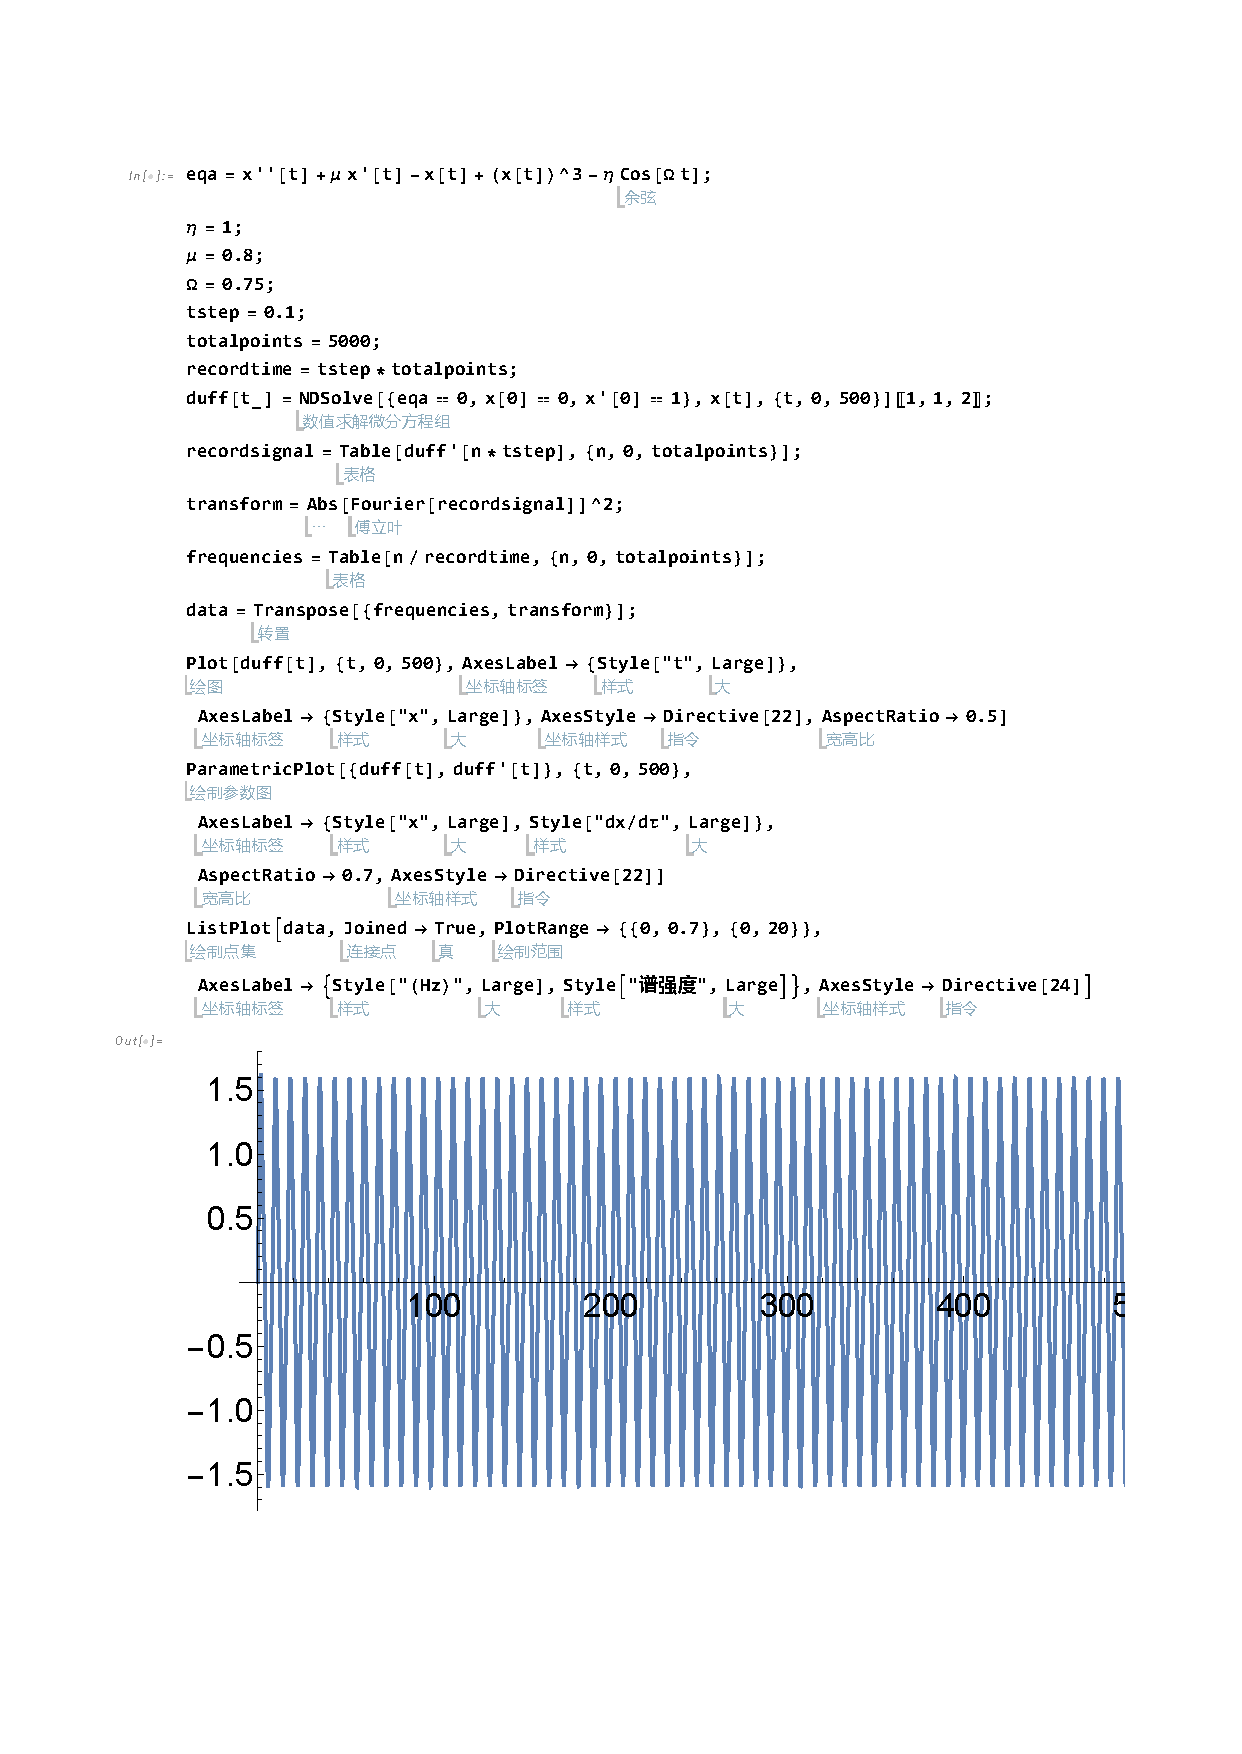
\includepdf[pages=-]{chaos.pdf}
%\subsection*{原件}
%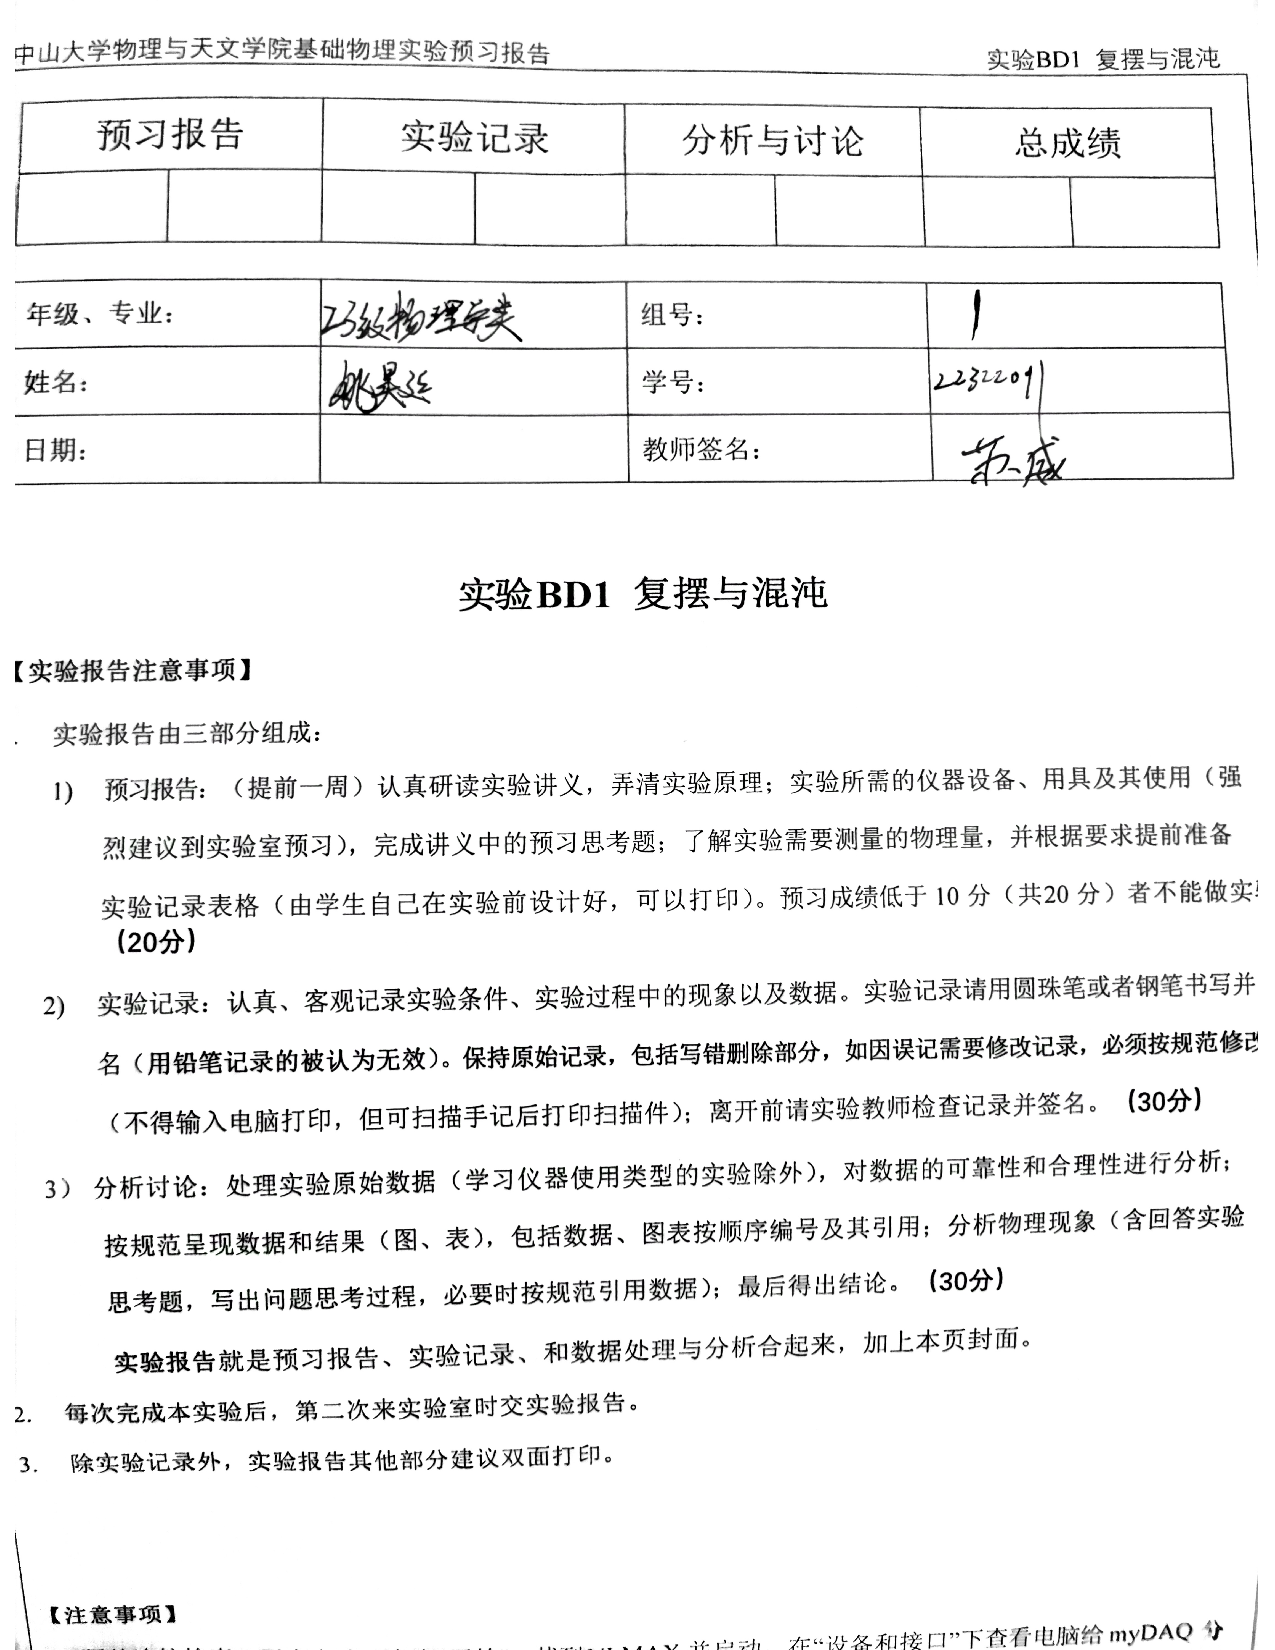
\includepdf[pages=-]{实验3原件.pdf}
%\begin{figure}[H]
%	\centering
%	\includegraphics[width=\textwidth]{焦距数据.jpg}
	
%\end{figure}
%\begin{figure}[H]
%	\centering
%	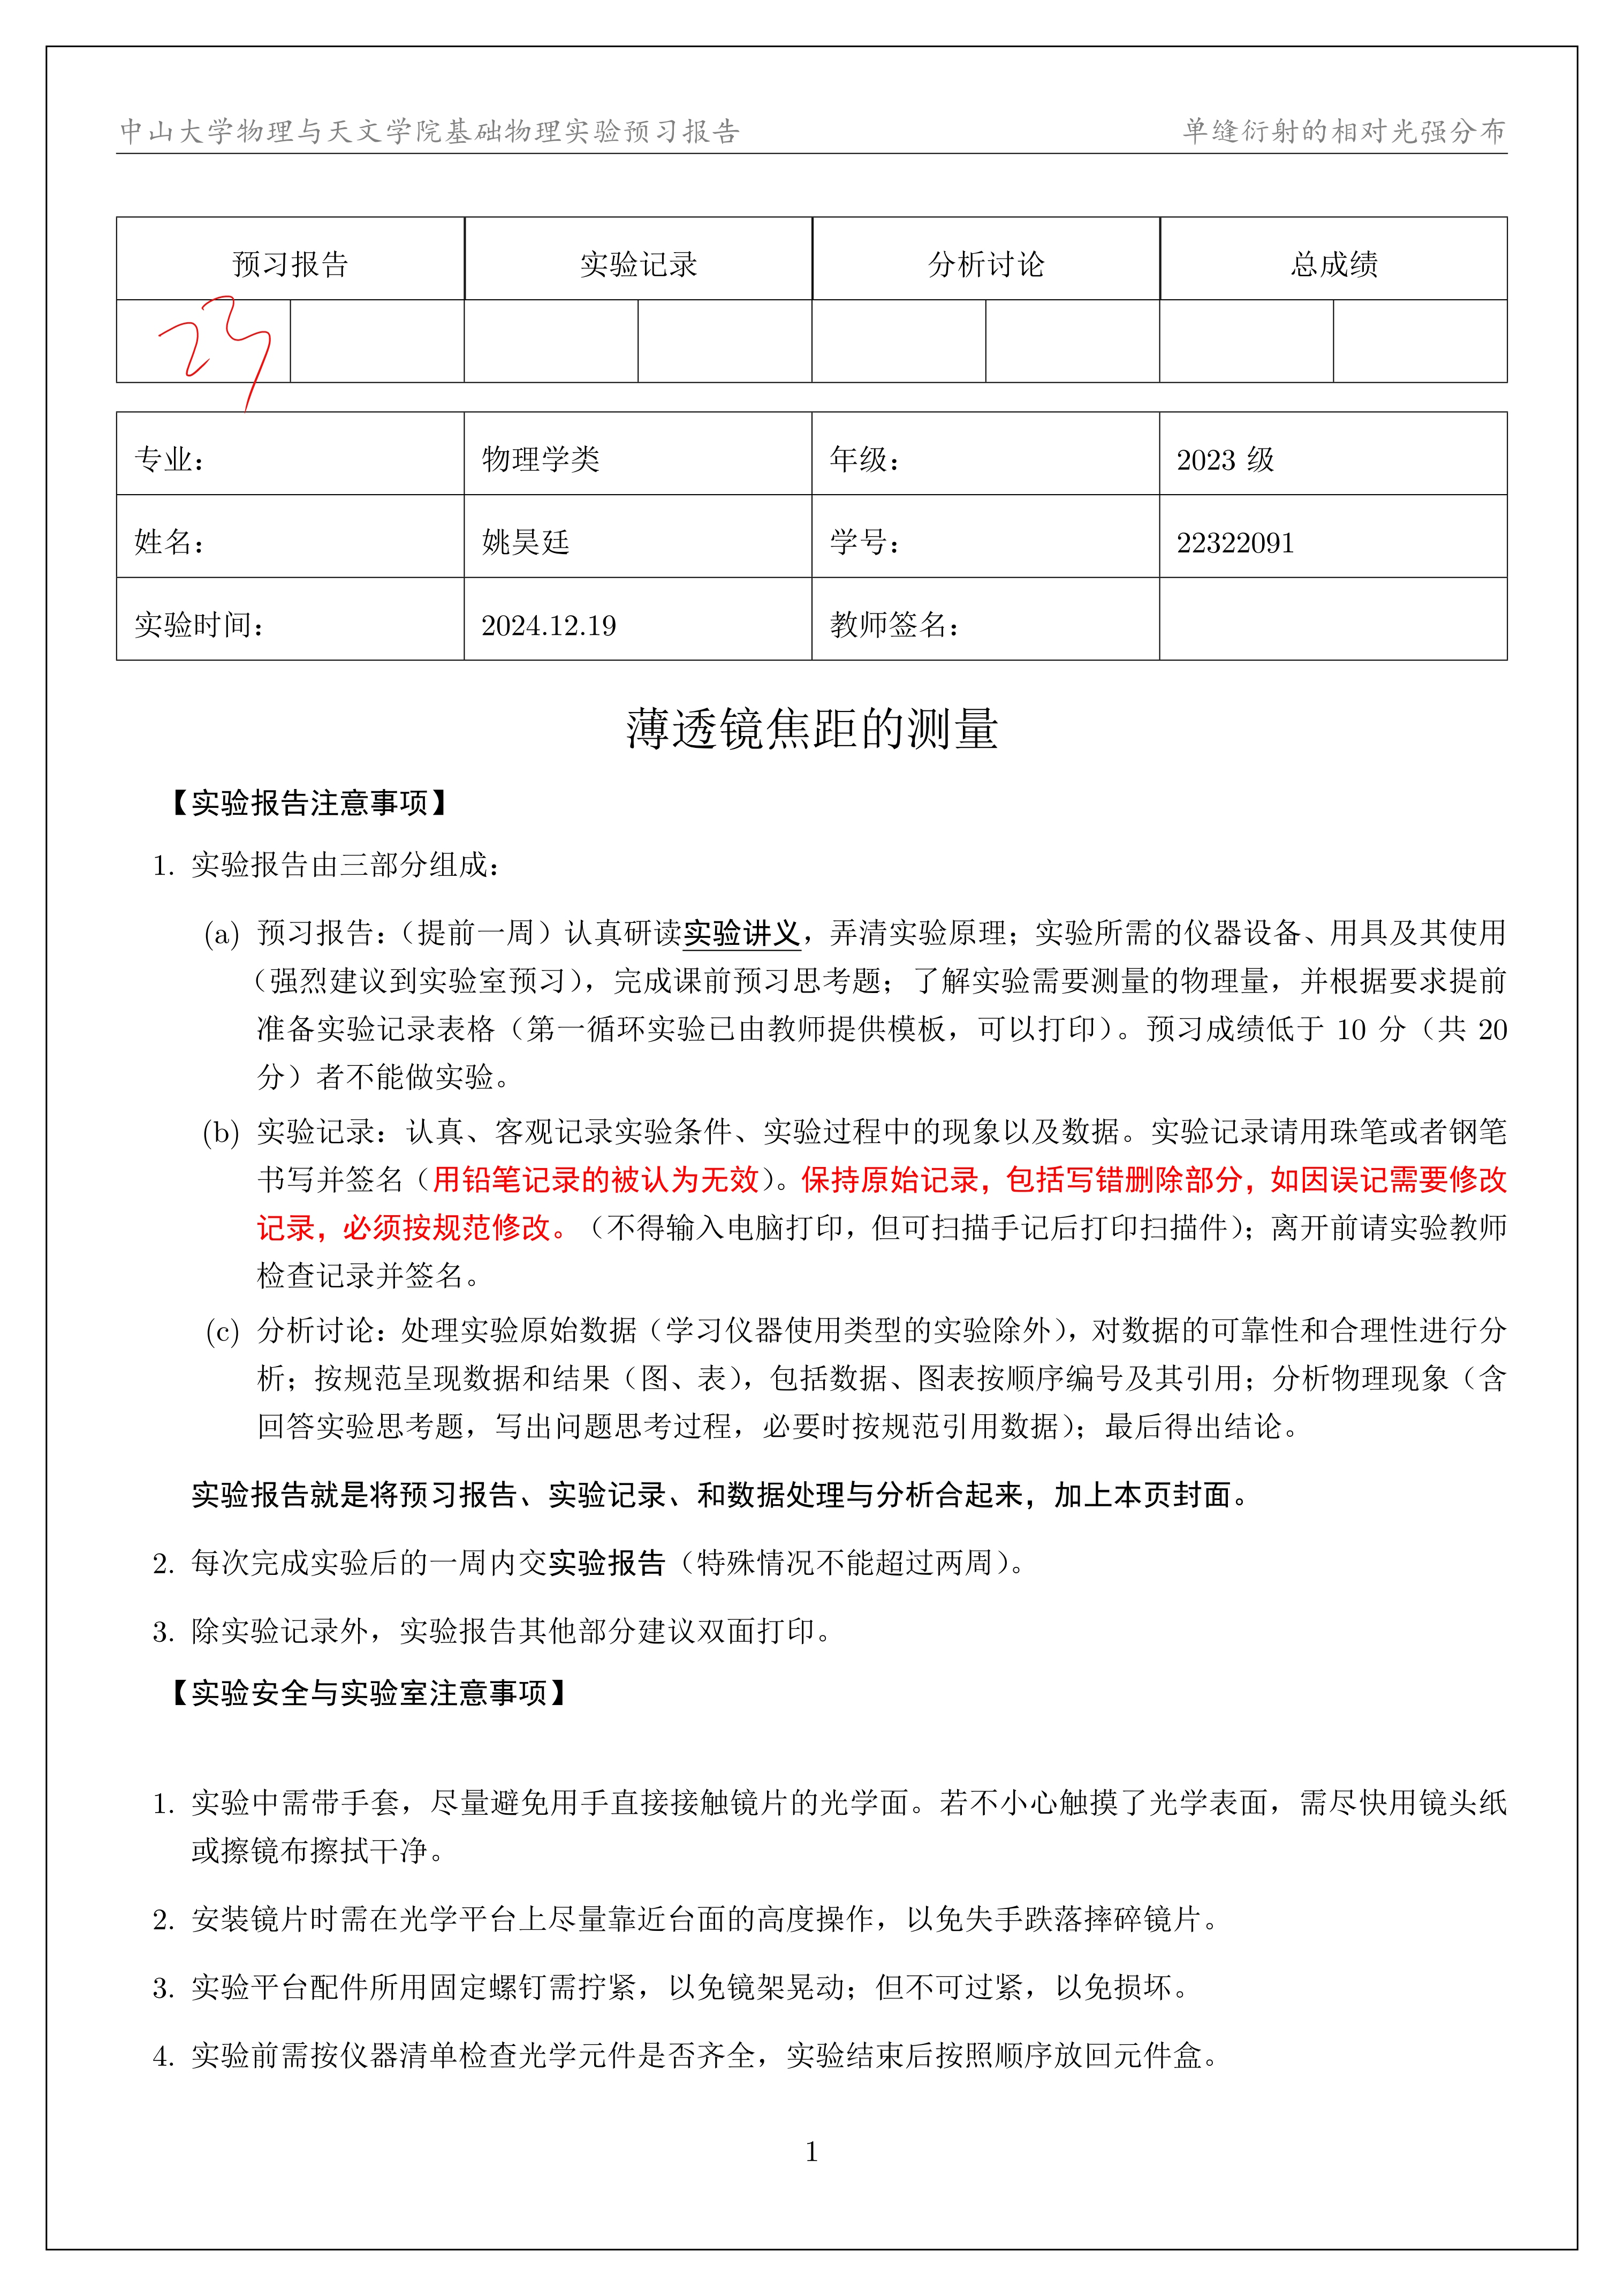
\includegraphics[width=\textwidth]{透镜焦距.jpg}
	
%\end{figure}

%\begin{figure}[H]
%	\centering
%	\includegraphics[width=0.4\textwidth]{单缝原件1.jpg}
%	\includegraphics[width=0.4\textwidth]{单缝原件2.jpg}
%	\includegraphics[width=0.4\textwidth]{单缝原件3.jpg}
%	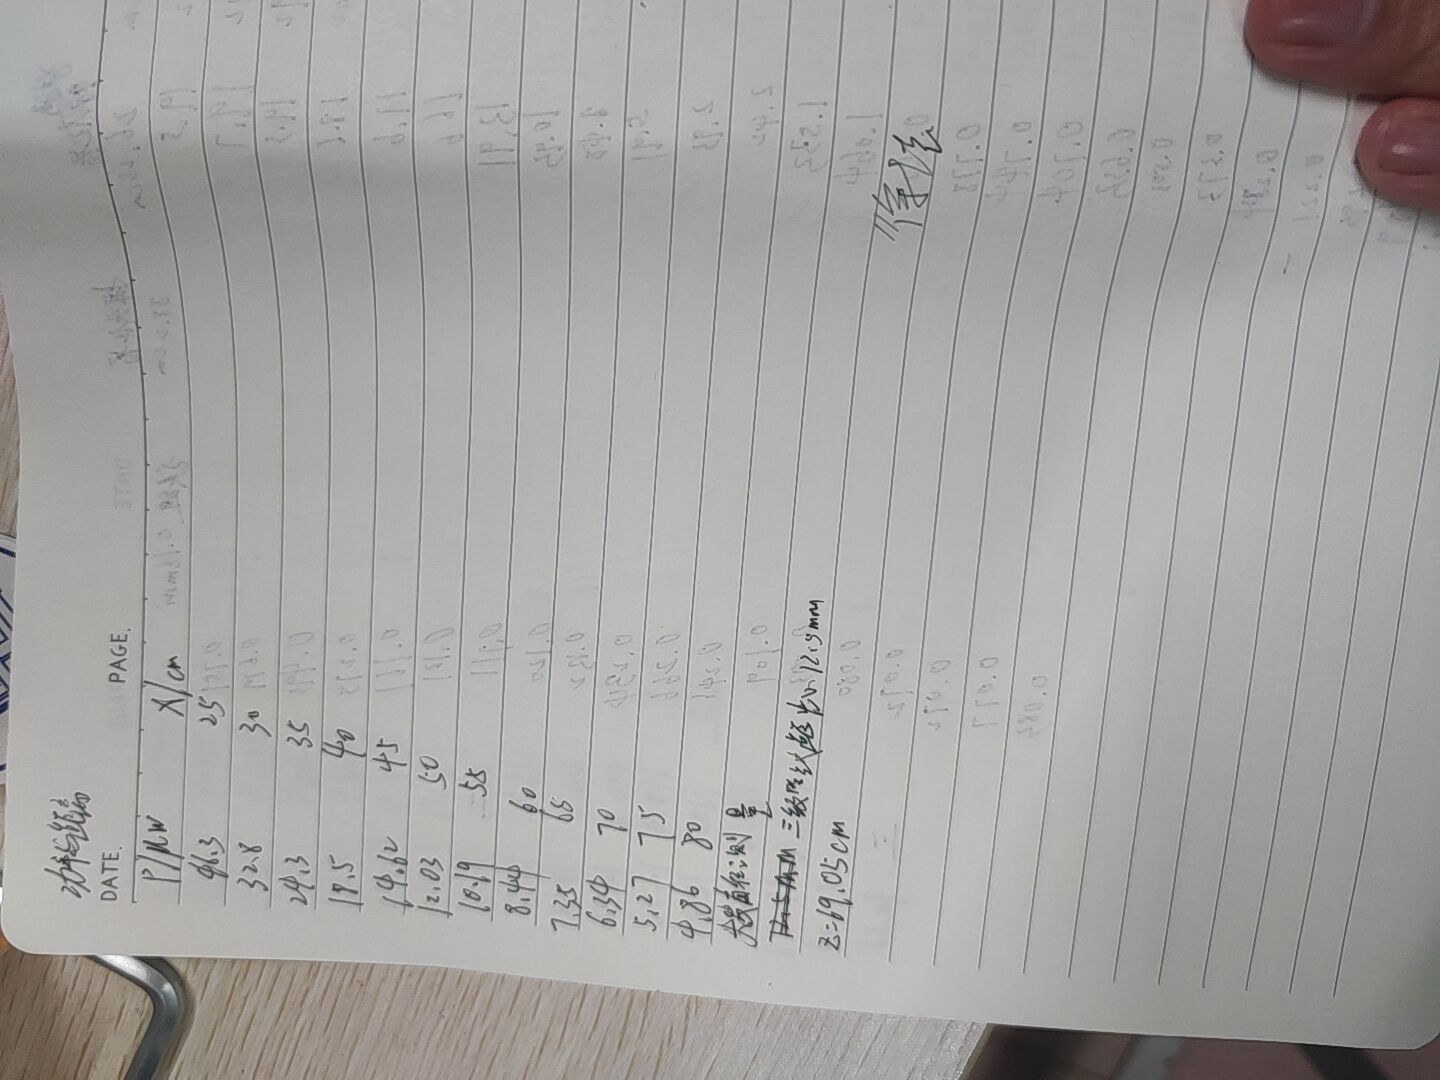
\includegraphics[width=0.4\textwidth]{单缝原件4.jpg}
%\end{figure}
%\subsection*{桌面}
%\begin{figure}[H]
%	\includegraphics[width=0.95\textwidth]{焦距桌面.jpg}
%\end{figure}
\end{document}
%